\documentclass[letterpaper,11pt]{article}
\oddsidemargin -1.0cm \textwidth 17.5cm

\usepackage[utf8]{inputenc}
\usepackage[activeacute,spanish, es-lcroman]{babel}
\decimalpoint
\usepackage{amsfonts,setspace}
\usepackage{amsmath}
\usepackage{amssymb, amsmath, amsthm}
\usepackage{comment}
\usepackage{float}
\usepackage{amssymb}
\usepackage{dsfont}
\usepackage{anysize}
\usepackage{multicol}
\usepackage{enumerate}
\usepackage{graphicx}
\usepackage[left=1.5cm,top=2cm,right=1.5cm, bottom=1.7cm]{geometry}
\setlength\headheight{1.5em} 
\usepackage{fancyhdr}
\usepackage{multicol}
\usepackage{hyperref}
\usepackage{wrapfig}
\usepackage{subcaption}
\usepackage{siunitx}
\usepackage{cancel}
\usepackage{mdwlist}
\usepackage{svg}
\pagestyle{fancy}
\fancyhf{}
\renewcommand{\labelenumi}{\normalsize\bfseries P\arabic{enumi}.}
\renewcommand{\labelenumii}{\normalsize\bfseries (\alph{enumii})}
\renewcommand{\labelenumiii}{\normalsize\bfseries \roman{enumiii})}


\begin{document}

\fancyhead[L]{\itshape{Facultad de Ciencias F\'isicas y Matem\'aticas}}
\fancyhead[R]{\itshape{Universidad de Chile}}
\rfoot[]{pág. \thepage}

\begin{minipage}{11.5cm}
    \begin{flushleft}
        \hspace*{-0.6cm}\textbf{FI1000 Introducción a la Física Clásica}\\
        \hspace*{-0.6cm}\textbf{Tutor:} Alejandro Cartes
    \end{flushleft}
\end{minipage}

\begin{picture}(2,3)
    \put(366, -10){
\includegraphics[scale=0.9]{2020-1/Imágenes/logo/dfi-fcfm.pdf}}
\end{picture}

\begin{center}
	\LARGE\textbf{Tutoría C3}\\
	\Large{Energía, Momentum, Centro de Masa y Colisiones}
\end{center}

\vspace{-1cm}
\begin{enumerate}\setlength{\itemsep}{0.4cm}

\item[]

\item 
\begin{multicols}{2}
Una masa $m$ se suelta en una pendiente con un ángulo de inclinación $\theta$ a una distancia $d$ de un resorte de constante elástica $k$ y un largo natural $\ell_0$ desconocido. Si los coeficientes de fricción estático y cinético entre la masa y la pendiente son $\mu_e$ y $\mu_c$ respectivamente. Determine:
    \begin{enumerate}
        \item La rapidez de la masa justo antes de llegar al resorte

        \item La compresión máxima del resorte

        \item Si la masa rebota hacia arriba, ¿qué tanto se acerca a su posición inicial?
    \end{enumerate}

\columnbreak
\begin{figure}[H]
    \centering
    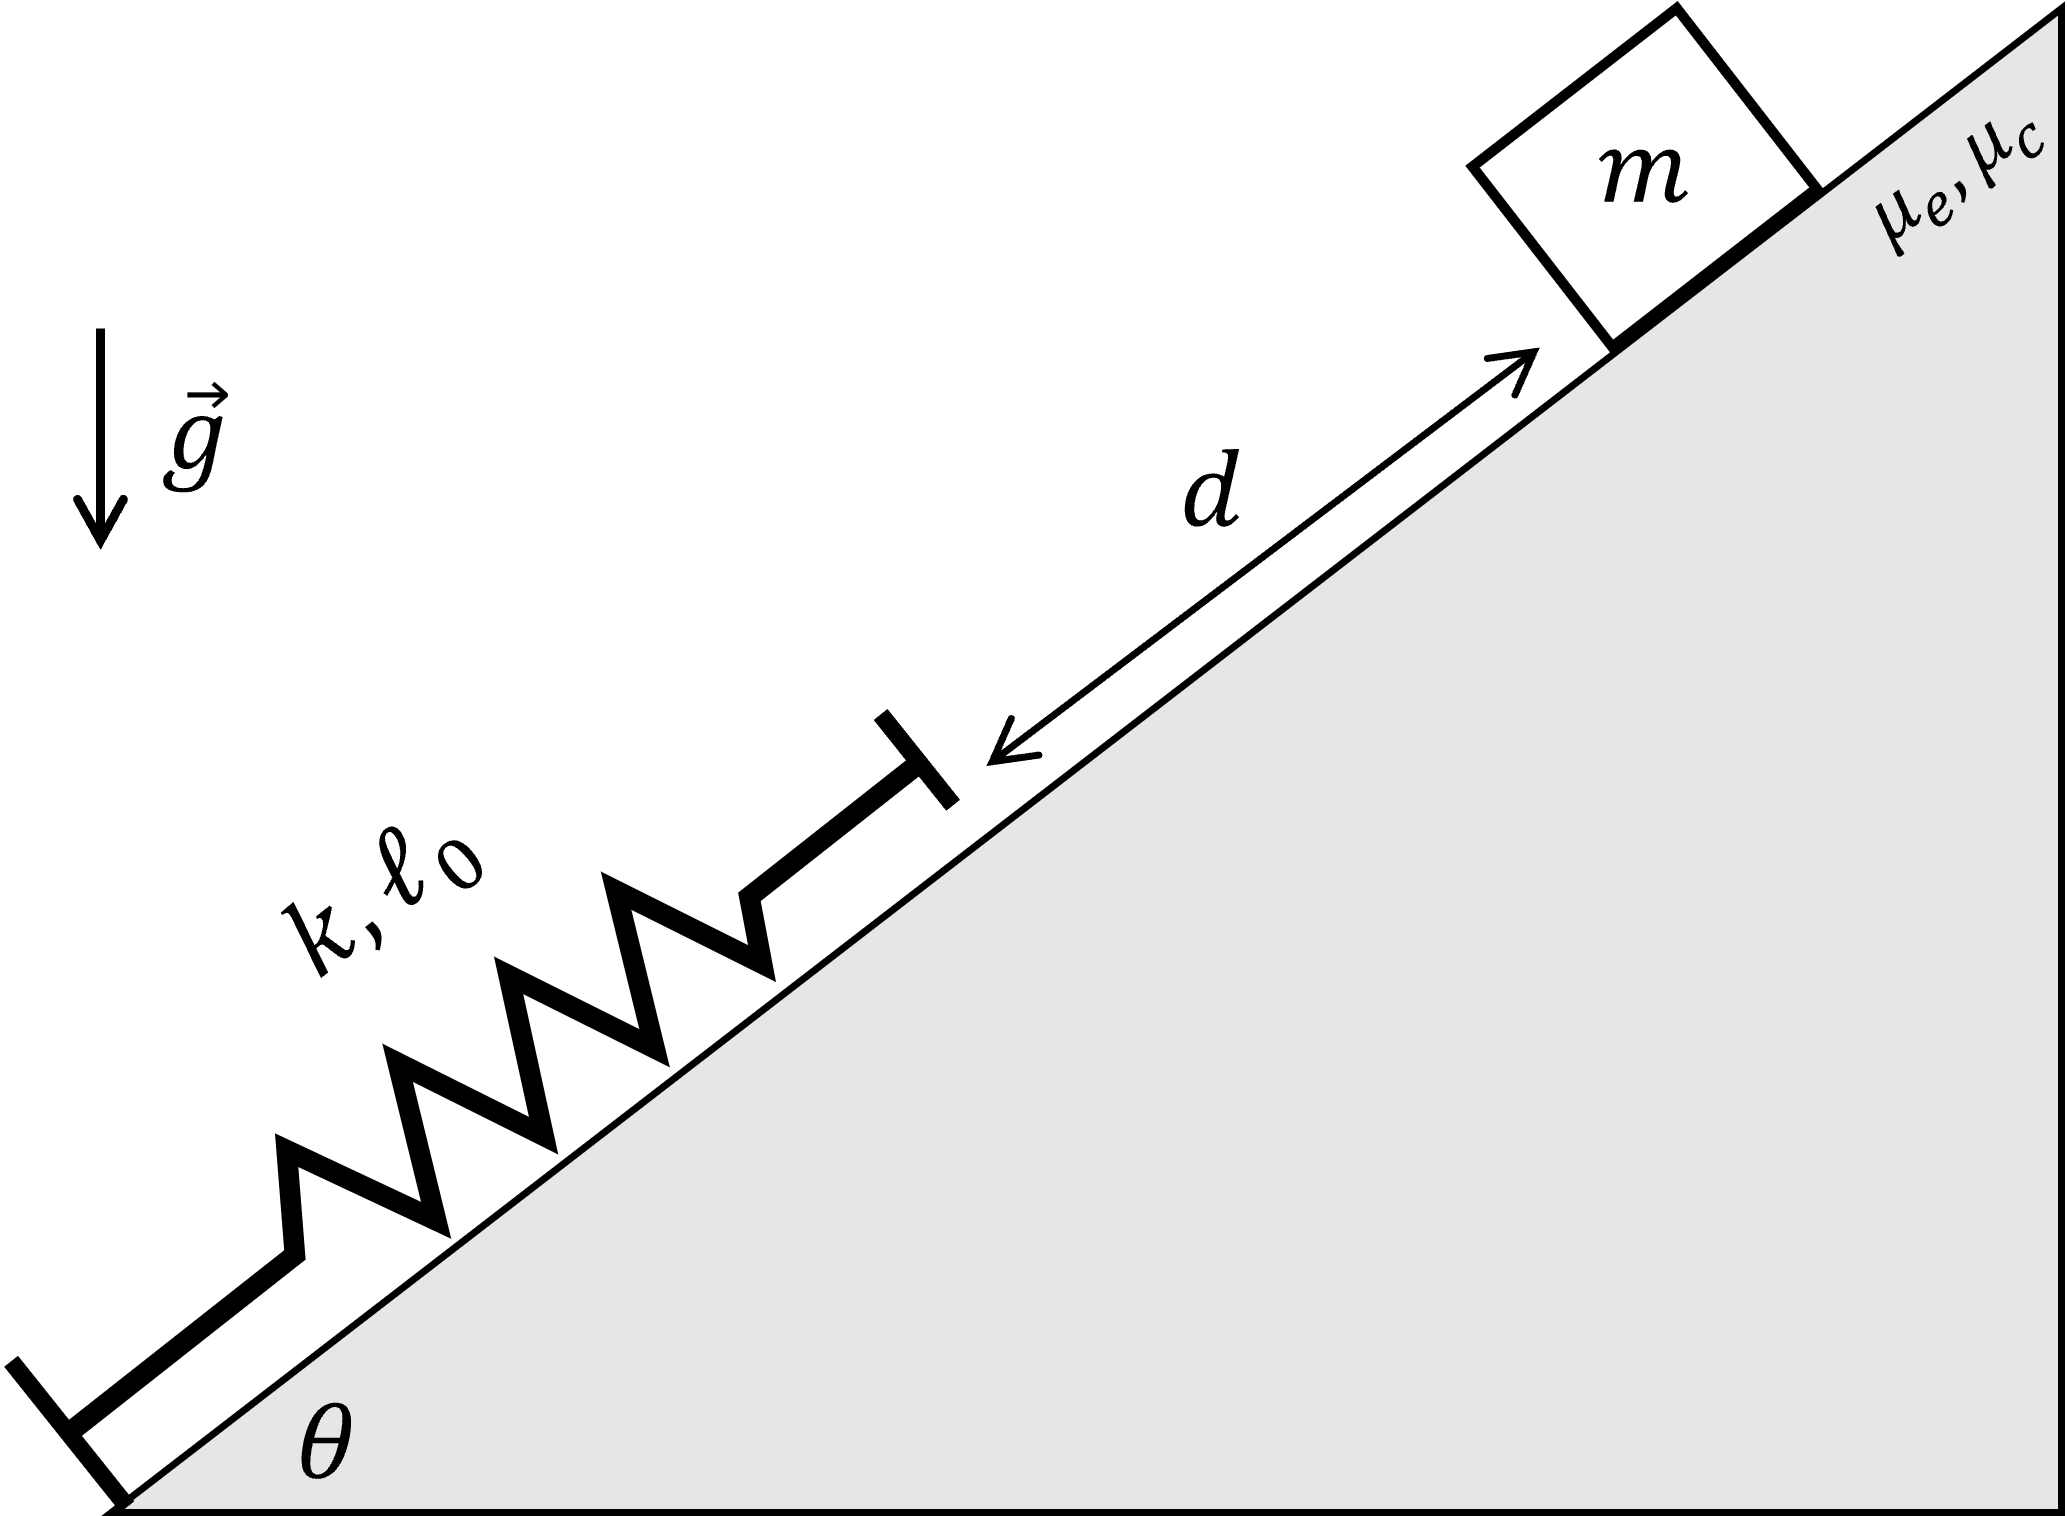
\includegraphics[width=0.8\linewidth]{tutorías/2023/img/tut-plano.png}
\end{figure}
\end{multicols}

\item \textbf{[P2-C3 2017-1]} Un bloque de masa $M$ con una superficie superior con la forma de medio cilindro de radio $R$ se encuentra sobre una superficie horizontal sin rozamiento al tiempo que toca un muro vertical en su lado izquierdo. Una partícula de masa $m$ se suelta desde el extremo superior izquierdo de la cavidad como se muestra en la figura. Suponiendo que la fricción puede despreciarse:
\begin{enumerate}
    \item Determine la rapidez de la partícula al llegar por primera vez a la parte más baja de su trayectoria
    
    \item Examine cualitativamente la acción de la fuerza normal del muro sobre el bloque de masa $M$ y determine el instante a partir del cual el bloque se desliza a la derecha. Para tiempos posteriores a este, ¿qué principio de conservación utiliza?
    
    \item Determine la rapidez máxima que alcanza el bloque en su movimiento después de soltar la masita $m$
\end{enumerate}


\begin{figure}[H]
    \centering
    \begin{subfigure}[t]{0.4\textwidth}
        \centering
        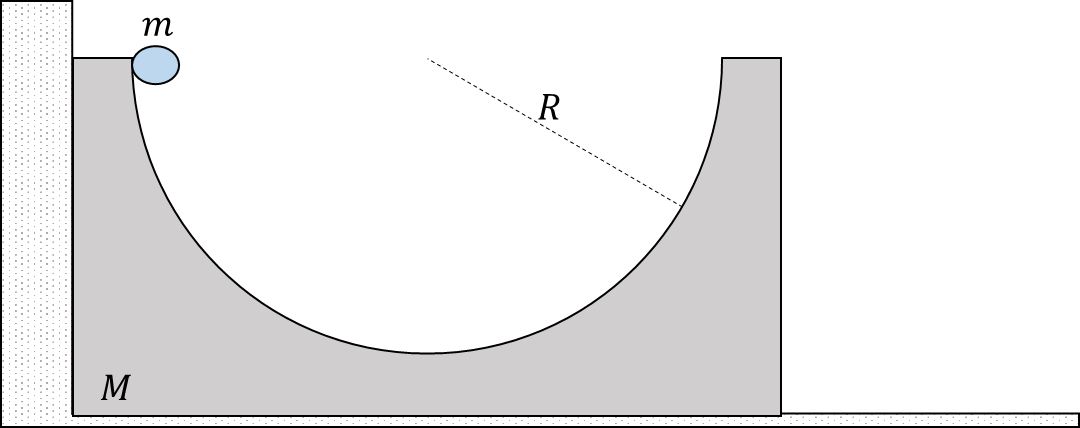
\includegraphics[width=1\linewidth]{2023-1/img/aux_11/bloque-p.png}
        \caption{P2}
    \end{subfigure}
    \hspace{2.5em}
    \begin{subfigure}[t]{0.4\textwidth}
        \centering
        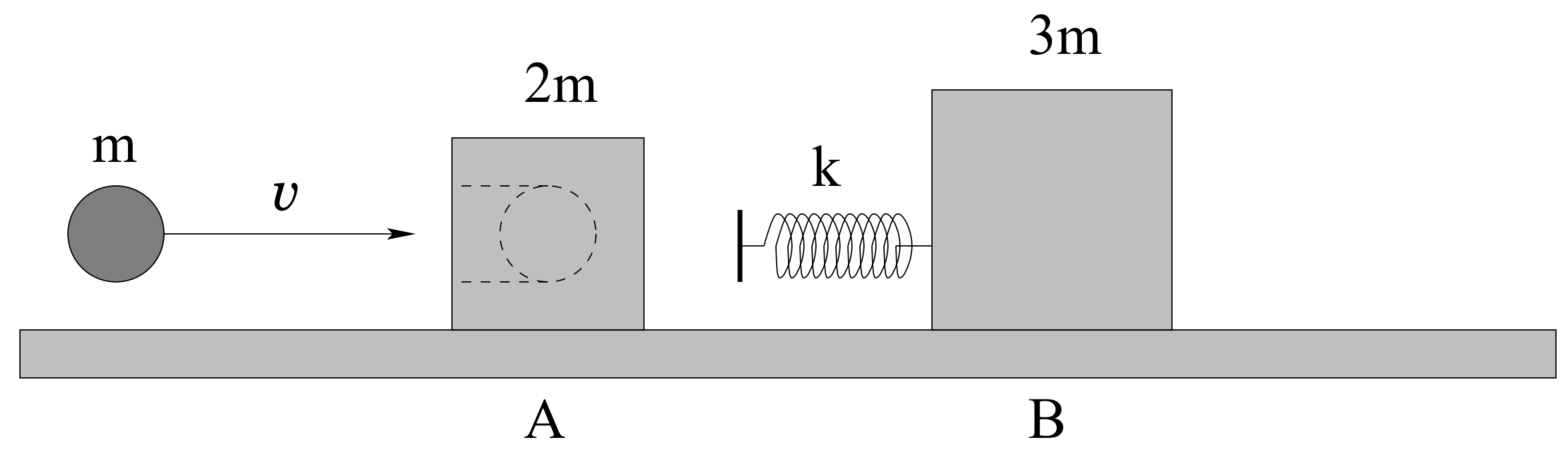
\includegraphics[width=1\linewidth]{tutorías/2023/img/tut-col.png}
        \caption{P3}
    \end{subfigure}
\end{figure}

\item Considere dos bloques $A$ y $B$, que se pueden mover sobre una superficie sin roce. El bloque $B$ tiene un resorte ideal de constante elástica $k$ y largo natural $\ell_0$ adherido. Una partícula que viaja con rapidez $v_0$ golpea al bloque $A$ quedando incrustada en este. Las masas de la partícula, $A$ y $B$ son $m$, $2m$ y $3m$ respectivamente.

    \begin{enumerate}
        \item ¿Está el sistema partícula-A-B aislado con respecto al momentum? ¿y con respecto a la energía? 
        \item ¿Cuál es la velocidad centro de masa del sistema? ¿varía o es constante?

        \item ¿Cuál es la velocidad del bloque $A$ inmediatamente después de ser golpeada por la partícula?

        \item ¿Cuál es la máxima compresión del resorte?
    \end{enumerate}

% Para imágenes vectoriales -> el texto tiene que estar en LaTeX
% \begin{figure}[htbp]
%   \centering
%   \svgpath{../Imagenes/ejercicios}  -> .. irse pa'trás 
%   \includesvg{ej5.svg}
% \end{figure}

\end{enumerate}
\end{document}
